\documentclass{article}

\usepackage{tikz}

\usepackage[english]{babel}
\usepackage[autostyle]{csquotes}
\MakeOuterQuote{"}

%\usepackage[T1]{fontenc}
%\usepackage[utf8]{inputenc}
%\usepackage{babel}
%\defineshorthand{"}{\textquotedbl}
\begin{document}
  All complete\footnote{A "complete" formula is one where the types of all free variables are known.} formulas of CoC can be immediately\footnote{By a process that is $O(n)$ in the size of the formula.} classified into one of the following groups.

  \vspace{0.5cm}

  \noindent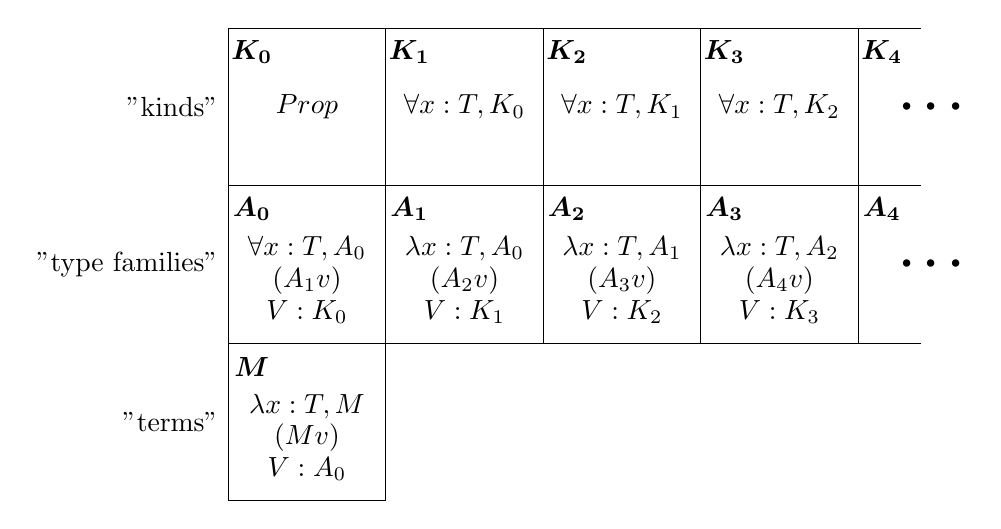
\begin{tikzpicture}
    \pgfsetxvec{\pgfpoint{2cm}{0}}
    \pgfsetyvec{\pgfpoint{0}{-2cm}}

    \draw (0,0.5) node[left]{"kinds"};
    \draw (0,1.5) node[left]{"type families"};
    \draw (0,2.5) node[left]{"terms"};
    \foreach \y in {0,1,2} {
      \draw (0,\y) rectangle (1,\y+1);
      \draw (4,\y) -- (4.4,\y);
    }
    \foreach \y in {0,1} {
      \draw (4.2,\y+0.5) node[right]{{\LARGE \boldmath $\cdots$}};
    }
    \foreach \x in {0,1,2,3,4} {
      \draw (\x+0.15,0.15) node[]{{\boldmath $K_\x$}};
      \draw (\x+0.15,1.15) node[]{{\boldmath $A_\x$}};
    }
    \foreach \x in {0,1,2,3} {
      \draw (\x+0.5,1.8) node[]{$V : K_\x$};
    }
    \draw (0.15,2.15) node[]{{\boldmath $M$}};
    \draw (0.5,0.5) node[]{$Prop$};
    \draw (0.5,1.4) node[]{$\forall x:T,A_0$};
    \draw (0.5,1.6) node[]{$(A_1 v)$};
    \draw (0.5,2.4) node[]{$\lambda x:T,M$};
    \draw (0.5,2.6) node[]{$(M v)$};
    \draw (0.5,2.8) node[]{$V : A_0$};
    \foreach \l/\x/\r in {0/1/2,1/2/3,2/3/4} {
%      \pgfmathsetmacro{\l}{\x-1};
      \draw (\x,0) rectangle (\x+1,1);
      \draw (\x+0.5,0.5) node[]{$\forall x:T,K_{\l}$};
      \draw (\x,1) rectangle (\x+1,2);
      \draw (\x+0.5,1.4) node[]{$\lambda x:T,A_{\l}$};
      \draw (\x+0.5,1.6) node[]{$(A_{\r} v)$};
    }
  \end{tikzpicture}

  \vspace{0.5cm}

  In the above chart, $V:T$ denotes a variable-usage-site whose bound type is in the cell $T$. The literal $T$ can denote any \emph{type}, and $v$ can denote any \emph{value}, which we shall define forthwith. The other letters refer to cells; for example, $A_2$ denotes any formula from the cell $A_2$.

  If\footnote{In general, it may be very difficult to determine whether a formula has a type \emph{at all}. But it is easy (again, $O(n)$) to give any formula $V$ a \emph{provisional} type $T$, where if $V$ has any types at all, its types are exactly all the well-typed beta-conversions of $T$. The only difficult part is determining whether function arguments have the correct types.} a formula has a type, that type is in the cell directly above its own. Thus, the \emph{values} (formulas that can be members of types) include everything except the top row, and the \emph{types} (formulas that can have members) include everything except the bottom-most cells. As such, $A_0$ (the cell of propositions) is the unique cell whose formulas are both types and values.
\end{document}
